\documentclass[9pt]{beamer}
\usepackage{kotex}
\usepackage{amsfonts,amssymb,amsthm}
\usepackage[dvipsnames]{xcolor}
\usepackage{xcolor}
\usepackage{etoolbox}
\usepackage{braket}
\usepackage{qcircuit}

%## color
\definecolor{customBlack}{HTML}{3B4252}
\definecolor{customBlackGrey}{HTML}{434C5e}
\definecolor{cuatomGrey}{HTML}{4C566A} 
\definecolor{customWhite}{HTML}{ECEFF4} 
\definecolor{customBlue}{HTML}{6082B6}  
\definecolor{customRed}{HTML}{BF616A}
\definecolor{vividauburn}{rgb}{0.58, 0.15, 0.14}


%## Theme & custom
% \usetheme{metropolis}           % Use metropolis theme
% \metroset{block=fill}
\usetheme{moloch} % modern fork of the metropolis theme
\molochset{block=fill}
\setbeamersize{text margin left=5mm, text margin right=5mm}
\setbeamercolor{palette primary}{bg=customBlack}
\setbeamercolor{alerted text}{fg=customRed}
\setbeamercolor{itemize item}{fg=customBlue}
\setbeamercolor{enumerate item}{fg=customBlue}


%## font
\usefonttheme[onlymath]{serif}
% \setbeamerfont{normal text}{size=\small}
% \setbeamerfont{math text}{size=\tiny}


%## Theorem title, numbering
\makeatletter
\setbeamertemplate{theorem begin}
{%
\begin{\inserttheoremblockenv}
{%
\inserttheoremheadfont
\inserttheoremname
\ifx\inserttheoremaddition\@empty\else\ of\ \inserttheoremaddition\fi%
\inserttheorempunctuation
}%
}
\setbeamertemplate{theorem end}{\end{\inserttheoremblockenv}}
\makeatother
\setbeamertemplate{theorems}[numbered]  


%## Custom block
\setbeamercolor{block title}{bg=customBlue, fg=white}
\setbeamercolor{block body}{bg=customWhite, fg=customBlack}
\setbeamercolor{block title alerted}{%
    use={block title, alerted text},
    bg=customRed,
    fg=white
}
\setbeamercolor{block body alerted}{%
    use={block title, alerted text},
    bg=customWhite,
    fg=customBlack
}
\AtBeginEnvironment{definition}{%
    \setbeamercolor{block title}{fg=white,bg=customBlackGrey}
    \setbeamercolor{block body}{fg=customBlack, bg=customWhite}
}
\AtBeginEnvironment{theorem}{%
    \setbeamercolor{block title}{fg=white,bg=customBlackGrey}
    \setbeamercolor{block body}{fg=customBlack, bg=customWhite}
}
\AtBeginEnvironment{corollary}{%
    \setbeamercolor{block title}{fg=white,bg=customBlackGrey}
    \setbeamercolor{block body}{fg=customBlack, bg=customWhite}
}
\AtBeginEnvironment{lemma}{%
    \setbeamercolor{block title}{fg=white,bg=customBlackGrey}
    \setbeamercolor{block body}{fg=customBlack, bg=customWhite}
}


%! Useful command
\renewcommand{\Pr}{\text{Pr}}
% $\ast$ \underline{Proof}:
%\checkmark \underline{meaning}:

\title{5. Quantum teleportation}
\date{\today}
\author{Vaughan Sohn}
% \institute{Centre for Modern Beamer Themes}


\begin{document}
    %#################################### 
    \maketitle
    
    %#################################### 
    \begin{frame}
        \frametitle{Contents}
        \tableofcontents
    \end{frame}

    %#################################### 
    \begin{section}{Quantum teleportation}
        \begin{frame}
            \frametitle{Teleportation system}
            \textbf{Introduction}
            \begin{itemize}
                \item Communication, 통신에서는 도청자에게 정보가 노출되지 않도록 정보를 전달하는 것을 중요한 목표 중 하나로 여긴다.
                \item 이번 강의에서는 정보 전달을 어떻게 수행할 수 있을지를 classical solution인 \alert{one-time pad}와 one-time pad로부터 영감을 받은 quantum solution에 대해서 소개하고자한다. 
            \end{itemize}
            \vspace{0.4cm}
            \textbf{System}: 다음과 같은 상황을 가정하자.
            \begin{itemize}
                \item Alice가 Bob에게 (one-bit; qubit) secret message를 전송하고자한다.
                \item 공개된 채널을 통해 전송되는 message는 도청자가 가로채더라도 해독할 수 없도록 ciphertext로 인코딩 되어야하며, 수신자는 ciphertext로부터 원본 메시지를 알아낼 수 있어야한다.
                \item Alice와 Bob은 서로 통신을 위해 secret information을 공유한다. \\(e.g., secret key, e-bit ...)
            \end{itemize}
        \end{frame}

        \begin{frame}
            \frametitle{Classical solution: One-time pad}
            Classical communication에서는 \textbf{one-time pad}\footnote{서로 더해서 0이되는 bit를 각각 1번씩(one-time) 더해줌으로써(pad) 전송중일때는 비밀을 보장하고 각자 해독할 수 있도록 한다.}라는 단순한 방법으로 해결할 수 있다. 
            \begin{figure}
                \centering
                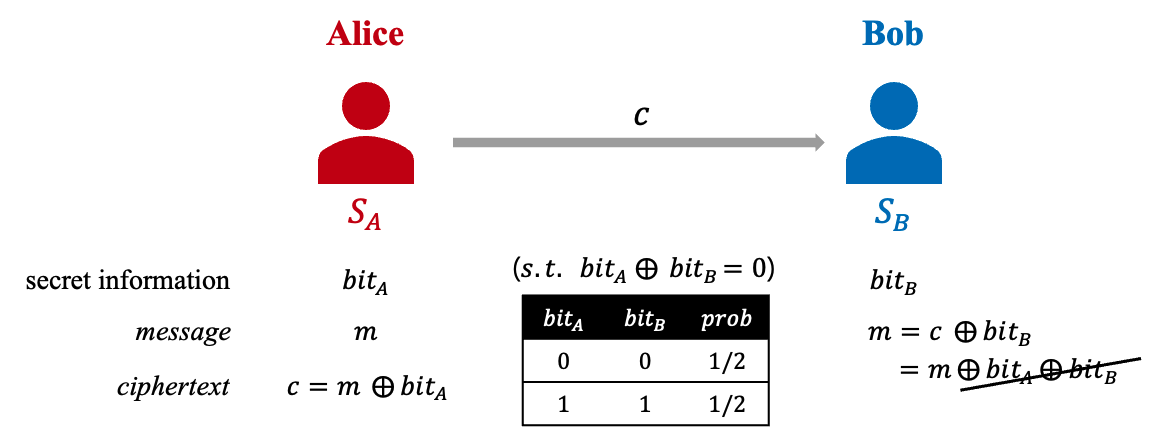
\includegraphics[width=0.95\textwidth]{image/L5_classical.png}
            \end{figure}
            \vspace{0.2cm}
            $\Rightarrow$ One-time pad로부터 아이디어를 얻어 secret message; \textbf{arbitrary quantum state}를 \alert{Classical Communication}만을 사용하여 전송하는 방법이 Quantum teleportation이다.
        \end{frame}


        \begin{frame}
            \frametitle{Quantum solution: Quantum teleportation}
            \textbf{System}
            \begin{itemize}
                \item message: Alice는 이제 Bob에게 \textit{quantum message} $\ket{\psi}$를 전송하려고 한다.
                \item secret information: Alice와 Bob은 서로 Bell-state $\ket{\Phi^+}$를 공유한다.\footnote{Bell state도 classical secret information처럼 "측정하면" $1/2$의 확률로 $\ket 0, \ket 0$이 되고 $1/2$의 확률로 $\ket 1, \ket 1$이 된다.}
            \end{itemize}
            \vspace{0.4cm}
            \textbf{Procedure}
            \begin{enumerate}
                \item Alice는 $\ket \psi$와 $\ket{\Phi^+}_A$를 measurement $M_{\Phi^+}$에 대해서 측정한다.
                \item Alice가 측정 결과로 얻은 2개의 classical bit를 전송한다.
                \item Bob은 전달받은 classical bit값에 따라 자신의 qubit $\ket{\Phi^+}_B$에 연산을 취한다.
                \begin{table}[]
                    \begin{tabular}{ccccc}
                        $\ket{\psi}$ &$\ket{\Phi^+}_A$ & prob &post state in $B$ &$U_B$\\\hline
                        0 & 0 & 1/4  & $\ket{\psi}$ & $I$ \\
                        0 & 1 & 1/4  & $\alpha \ket 1 + \beta \ket 0$ & $X$\\
                        1 & 0 & 1/4  & $\alpha \ket 0 - \beta \ket 1$ & $Z$\\
                        1 & 1 & 1/4  & $\alpha \ket 1 - \beta \ket 0$ & $ZX$ 
                    \end{tabular}
                    \end{table}
            \end{enumerate}
            $\Rightarrow$ \textbf{Bell measurement}와 \textbf{Classical Communication}만을 사용하여 arbitrary quantum state $\ket \psi$를 전송할 수 있다!
        \end{frame}
    \end{section}

    \begin{frame}
        \frametitle{Quantum solution: Quantum teleportation}
        앞에서 소개한 Quantum teleportation을 Quantum circuit으로 구현하면 다음과 같다.
        \begin{figure}
            \centering
            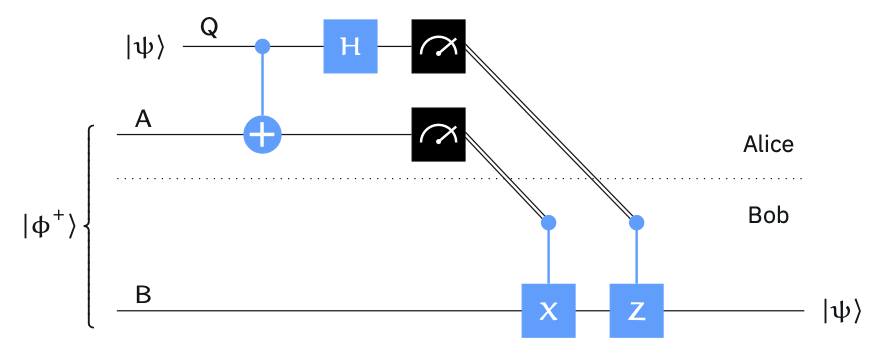
\includegraphics[width=0.9\textwidth]{image/L5_quantum.png}
        \end{figure}
    
    \end{frame}
    %#################################### 
    \begin{frame}{Summary}
        \begin{block}{Summary}
            \begin{itemize}
                \item Classical communication에서는 더해서 0이 되는 secret bit를 공유하여 communication을 수행한다.
                \item QUantum communication에서는 entangled-qubit을 서로 공유한뒤, message와 함께 Bell measurement를 수행한 결과를 Classical communication으로 전송하여 quantum state를 전송할 수 있다.
            \end{itemize}
        \end{block}
    \end{frame}


    %#################################### 
    \begin{frame}{References}
        \begin{itemize}
            \item Lecture notes for EE547: Introduction to Quantum Information Processing (Fall 2024)
        \end{itemize}
        \vspace{6cm}
    \end{frame}


\end{document}